\begin{figure}
  \centering
  \vskip -0.25cm
  \begin{tikzpicture}    
    \node at (0, 0){
      \includegraphics[width=6cm]{experiments/3d/vae_occ_aml/moderate_15/results_0}
    };
    \node at (0, -2.75) {
      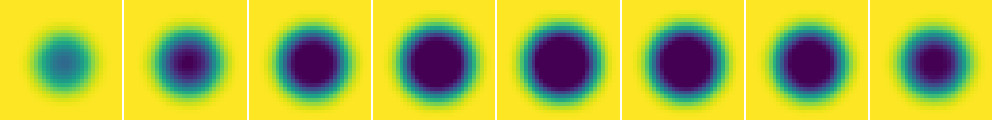
\includegraphics[width=6cm]{experiments/3d/vae_occ_aml/inference_statistics_05}
    };
    \node at (0, -5.25){
      \includegraphics[width=6cm]{experiments/3d/vae_occ_aml/hard_15_statistics_05/results_0}
    };
    \node at (0, -9.75){
      \includegraphics[width=6cm]{experiments/3d/vae_evae/hard_15_statistics/results_0}
    };
    
    %\draw[-,dashed] (3.25, -3) -- (3.25,3);
    
    \node at (6.5, 0){
      \includegraphics[width=6cm]{experiments/3d/vae_occ_aml/moderate_15/results_1}
    };
    \node at (6.5, -2.75) {
      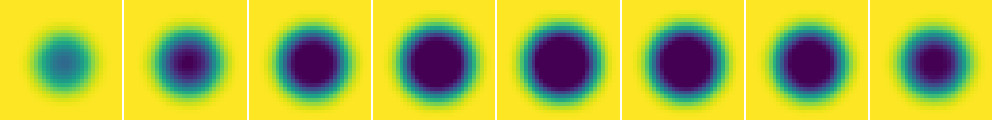
\includegraphics[width=6cm]{experiments/3d/vae_occ_aml/inference_statistics_05}
    };
    \node at (6.5, -5.25){
      \includegraphics[width=6cm]{experiments/3d/vae_occ_aml/hard_15_statistics_05/results_1}
    };
    \node at (6.5, -9.75){
      \includegraphics[width=6cm]{experiments/3d/vae_evae/hard_15_statistics/results_1}
    };
    
    \node at (10,0) {
      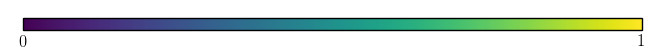
\includegraphics[height=4.25cm]{experiments/3d/vae_occ/easy_15/colorbar}
    };
   
    \draw[-,dashed] (-3.5,-2.125) -- (10,-2.125);
    \draw[-,dashed] (-3.5,-7.5) -- (10,-7.5);
    
    \node[rotate=90] at (-4, 0) {\begin{tabular}{c}\AML\\\moderate\end{tabular}};
    \node[rotate=90] at (-4, -4.25) {\begin{tabular}{c}\AML\\\hard\end{tabular}};
    \node[rotate=90] at (-4, -9.75) {\begin{tabular}{c}\EVAE\\\hard\end{tabular}};
    
  \end{tikzpicture}
  \vskip 6px
  
  % TODO short caption
  \caption{Qualitative results for \AML on the 3D cuboids dataset with a \VAE
  prior and $Q = 15$. We
  show results on \moderate and \hard difficulties in comparison with \EVAE.
  In all cases we show
  horizontal slices of the volumes, \ie heights $8 + 2i$ for $0 \leq i < 8$,
  for two samples samples,
  each showing the observed points, the partial free space, the target shape
  as well as the predicted shape and
  the corresponding error. For \AML and the hard case we additionally
  illustrate the weights $\rho_i$ that
  were used for both \AML and \EVAE.}
  \label{fig:experiments-3d-aml-qual-1}
\end{figure}
\begin{figure}
  \centering
  \vskip -0.25cm
  \begin{tikzpicture}    
    \node at (0, 0){
      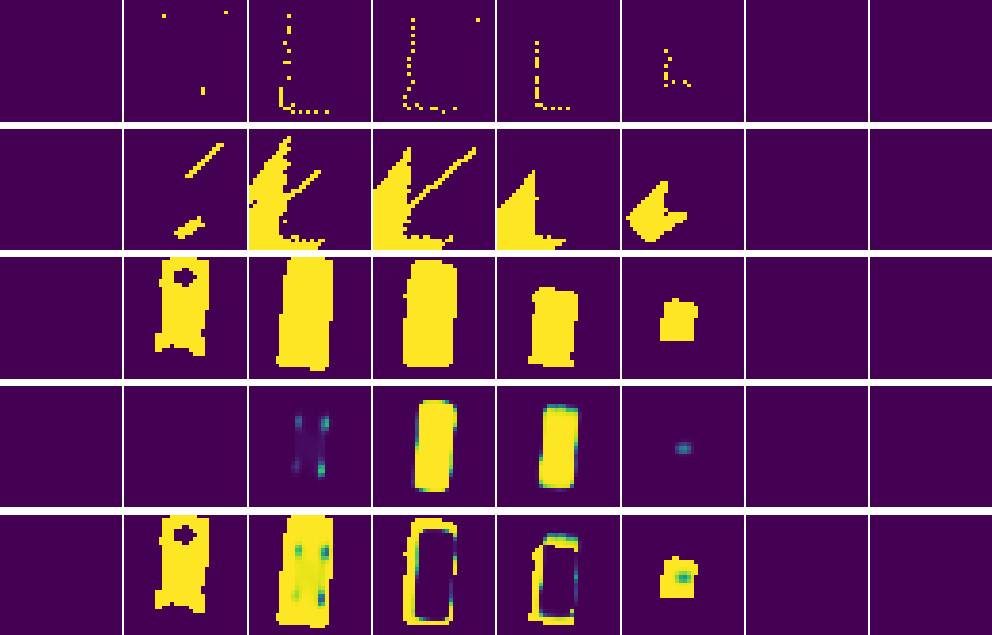
\includegraphics[width=6cm]{experiments/3d/vae_occ_sdf_aml/hard_15_statistics/results_0_0}
    };
    \node at (0, -4){
      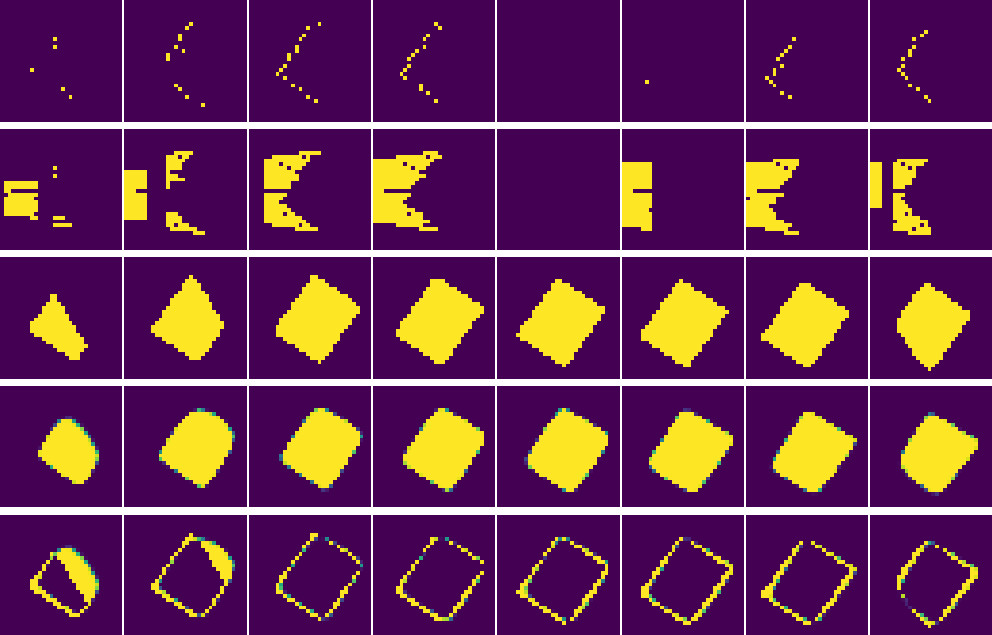
\includegraphics[width=6cm]{experiments/3d/vae_occ_sdf_aml/hard_15_statistics/results_1_0}
    };
    
    %\draw[-,dashed] (3.25, -3) -- (3.25,3);
    
    \node at (6.5, 0){
      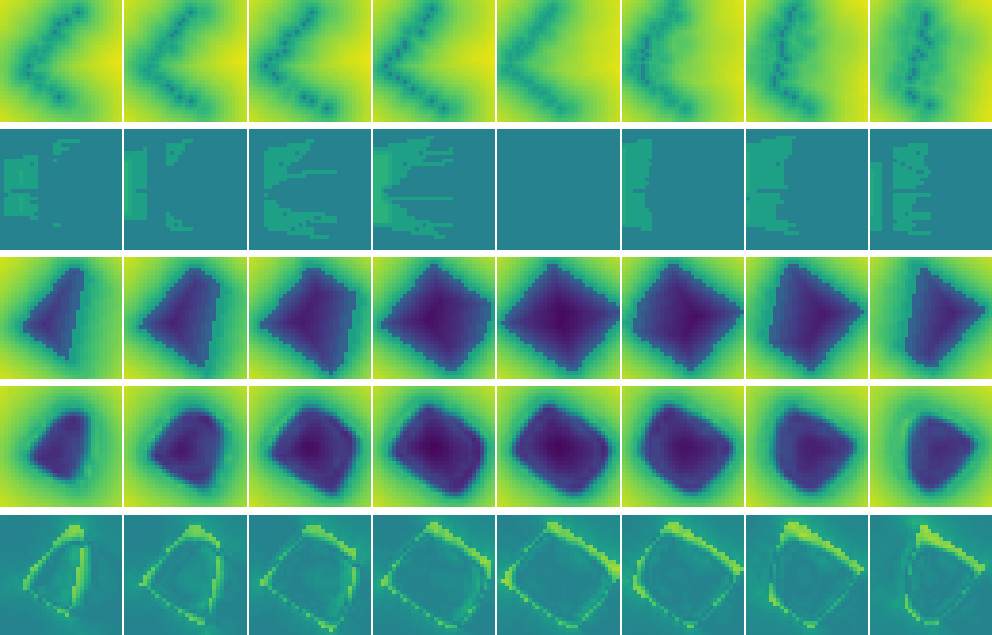
\includegraphics[width=6cm]{experiments/3d/vae_occ_sdf_aml/hard_15_statistics/results_0_1}
    };
    \node at (6.5, -4){
      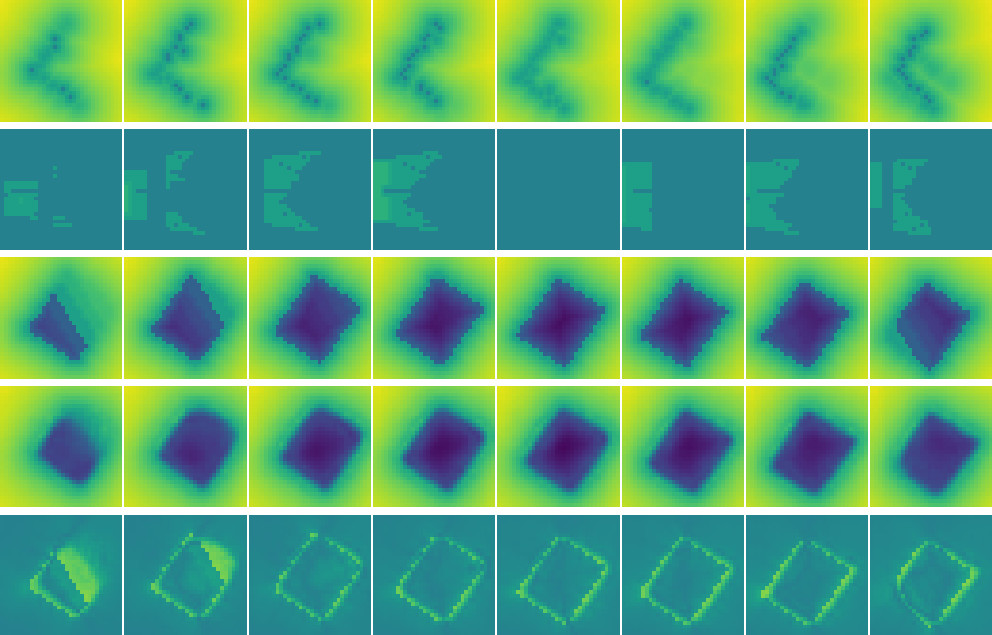
\includegraphics[width=6cm]{experiments/3d/vae_occ_sdf_aml/hard_15_statistics/results_1_1}
    };
    
    \node at (10,0) {
      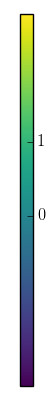
\includegraphics[height=4.25cm]{experiments/3d/vae_occ_sdf_aml/colorbar_1}
    };
    
    \node at (-3.5,0) {
      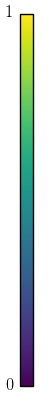
\includegraphics[height=4.25cm]{experiments/3d/vae_occ_sdf_aml/colorbar_0}
    };
    
    \node at (0, 2.25) {occupancy};
    \node at (6.5, 2.25) {signed distance function};
    
  \end{tikzpicture}
  \vskip 6px
  
  % TODO short caption
  \caption{Qualitative results for \AML using a \VAE prior with $Q = 15$ trained on both
  occupancy and signed distance functions. Results correspond to the \hard case.
  We show two samples and both modalities. In all
  cases we show horizontal slices as in Figure \ref{fig:experiments-3d-aml-qual-1}
  corresponding to the observed points, the partial free space, the target shape as well as the
  predicted shape and its error. We selected two examples illustrating that 
  the model resorts to blob-like ``standard'' shapes.}
  \label{fig:experiments-3d-aml-qual-2}
\end{figure}

